\section{Optimization Results} \label{sec: parameters results}

Our procedure has been making a grid with the four parameters of the robot 
design: $w$ (width of the cylinders), $N$(number of cylinders), $r_{wheel}$ and $r_{flywheel}$.
We have fixed $r_{flywheel}$ to a number of discrete values between 0.05 and 0.125 and, for each one, we evaluate the cost for each point of the grid,
remove those which do not fulfill the restrictions, and keep the configuration providing the minimum cost. 

\begin{figure}[H]
	\centering
	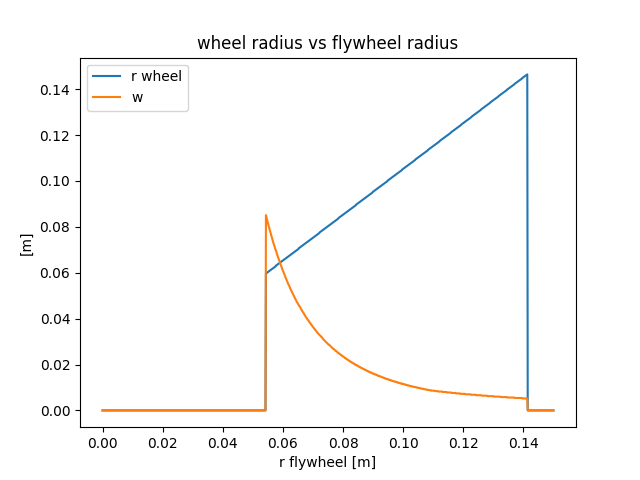
\includegraphics[width=10cm]{img/optimization/parameters.png}
	\caption{Plot of the wheel radius and the width of the cylinder that was optimal for each flywheel radius.}
	\label{fig:Parameters plot}
\end{figure}

We can observe that the relation between the flywheel radius and 
the wheel radius is linear. This is because we are always on the
edge of the restriction number one.

\begin{figure}[H]
	\centering
	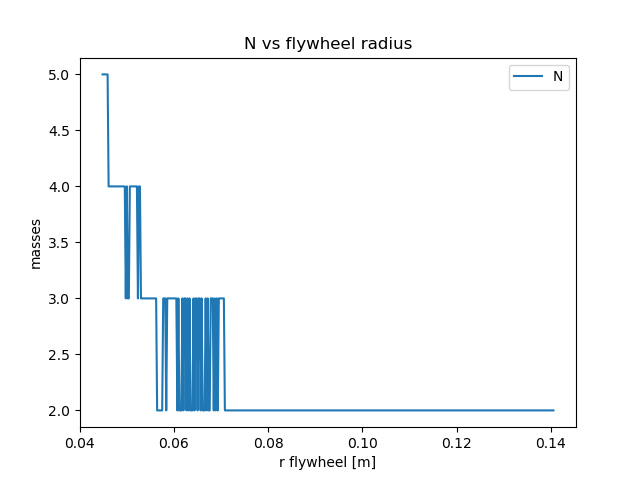
\includegraphics[width=10cm]{img/optimization/N.png}
	\caption{Plot of the N that minimize the cost function.}
	\label{fig:Parameters plot}
\end{figure}


\begin{figure}[H]
	\centering
	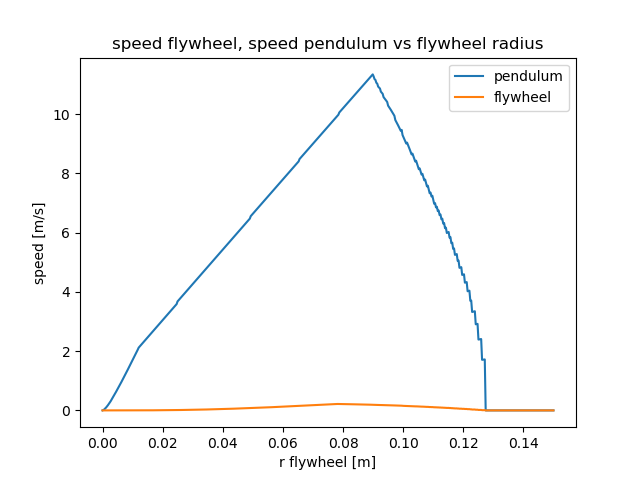
\includegraphics[width=10cm]{img/optimization/speed.png}
	\caption{Plot of the equations \ref{Maximum speed flywheel} and \ref{maximum speed pendulum} at the parameters that minimize the cost function and fullfil the requirements and restrictions}
	\label{fig:Speed plot}
\end{figure}

In this figure we can observe that the speed of in the pendulum mode increases
linearly with the flywheel radius. This is because it is linearly related with
the wheel radius.

\begin{figure}[H]
	\centering
	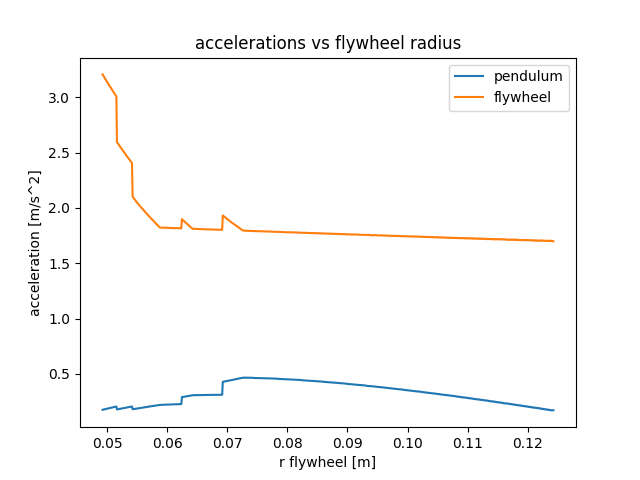
\includegraphics[width=10cm]{img/optimization/acceleration.png}
	\caption{Plot of the equations \ref{maximum acceleration flywheel} and \ref{maximum acceleration pendulum} at the parameters that minimize the cost and fulfill the requirements and restrictions}
	\label{fig:Speed plot}
\end{figure}

\begin{figure}[H]
	\centering
	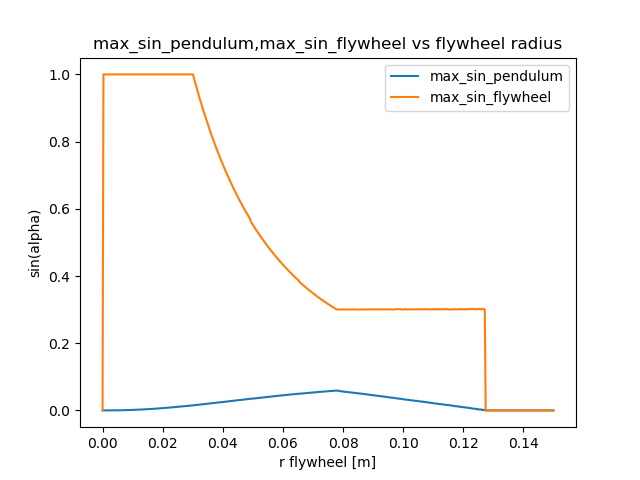
\includegraphics[width=10cm]{img/optimization/sin.png}
	\caption{Plot of the equations \ref{Maximum angle using flywheel system} and \ref{Maximum angle using pendulum system} at the parameters that minimize the cost and fulfill the requirements and restrictions}
	\label{fig:Sinus plot}
\end{figure}

We can see in figure \ref{fig:Sinus plot} that when the flywheel radius 
exceeds 0.07 m the requirement of the flywheel sinus becomes active.



\begin{figure}[H]
	\centering
	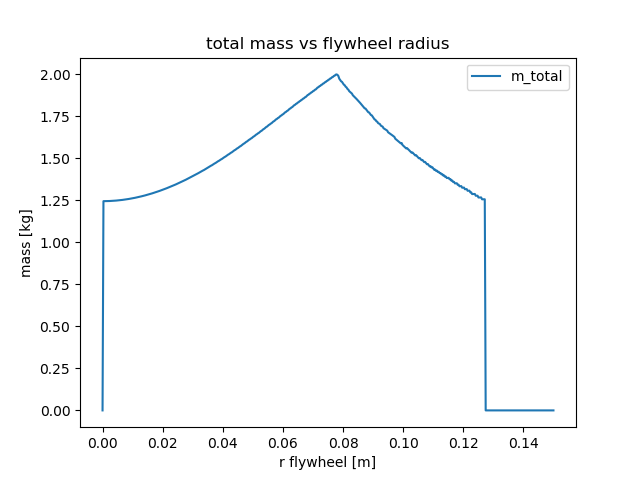
\includegraphics[width=10cm]{img/optimization/mass.png}
	\caption{Plot of the mass for each configuration.}
	\label{fig:Mass plot}
\end{figure}

We can see in figure \ref{fig:Mass plot} that the total mass never exceeds the
5 kg limit.

%\begin{figure}[H]
%	\centering
%	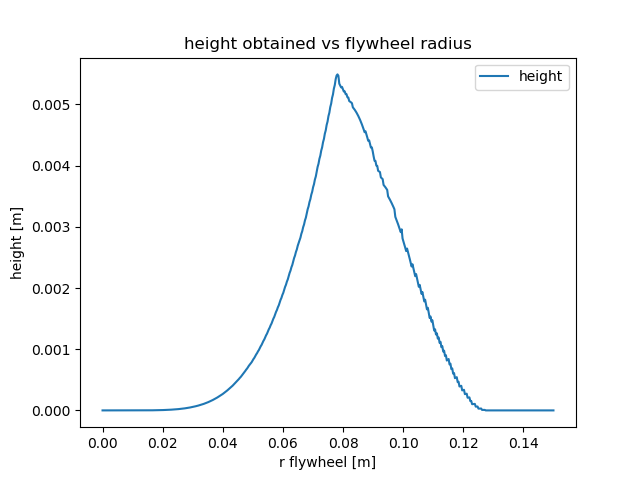
\includegraphics[width=10cm]{img/optimization/height.png}
%	\caption{Plot of the equation \ref{Maximum height} for each configuration.}
%	\label{fig:Mass plot}
%\end{figure}

\begin{figure}[H]
	\centering
	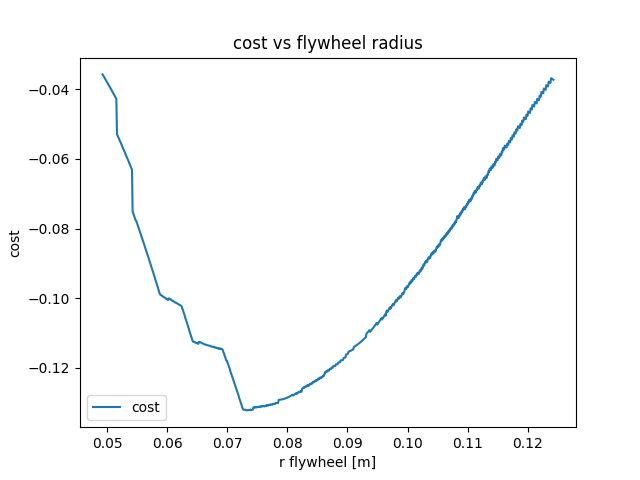
\includegraphics[width=10cm]{img/optimization/cost.png}
	\caption{Plot of the equation \ref{eq: cost} for each configuration.}
	\label{fig:Cost plot}
\end{figure}

Seeing the parameters that minimize cost and the material that we had available
our selected parameters were:
\begin{center}
	\begin{tabular}{ |c|c|c|c| } 
	 \hline
	 $r_{flywheel}$ & $r_{wheel}$ & $w$ & $N$\\
	 \hline 
	 8cm & 10cm & 5cm & 2 \\ 
	 \hline
	\end{tabular}
\end{center}

With these parameters we get the following specifications:
\begin{center}
	\begin{tabular}{ |c|c| } 
	 \hline
	 Total mass & 2,91 kg\\
	 \hline
	 \textbf{Pendulum} \\
	 \hline
	 Maximum sinus & 0,042\\
	 \hline
	 Maximum speed horizontal & 1,84 $m/s$\\
	 \hline
	 Maximum acceleration horizontal & 0,38 $m/s^2$\\
	 \hline
	 \textbf{Flywheel} \\
	 \hline
	 Maximum sinus & 0,171\\
	 \hline
	 Maximum speed horizontal & 0,24 $m/s$\\
	 \hline
	 Maximum acceleration horizontal & 1.52 $m/s^2$\\
	 \hline
	\end{tabular}
\end{center}